%% Le lingue utilizzate, che verranno passate come opzioni al pacchetto babel. Come sempre, l'ultima indicata sarà quella primaria.
%% Se si utilizzano una o più lingue diverse da "italian" o "english", leggere le istruzioni in fondo.
\def\thudbabelopt{english,italian}
%% Valori ammessi per target: bach (tesi triennale), mst (tesi magistrale), phd (tesi di dottorato).
%% Valori ammessi per aauheader: '' (vuoto -> nessun header Alpen Adria Univeristat), aics (Department of Artificial Intelligence and Cybersecurity), informatics (Department of Informatics Systems). Il nome del dipartimento è allineato con la versione inglese del logo UniUD.
\documentclass[target=mst,aauheader=]{thud}
\graphicspath{ {./images/} }

%% --- Informazioni sulla tesi ---
%% Per tutti i tipi di tesi
% Scommentare quello di interesse, o mettete quello che vi pare
\course{Informatica}
%\course{Internet of Things, Big Data e Web}
%\course{Matematica}
%\course{Comunicazione Multimediale e Tecnologie dell'Informazione}
\title{Vulnerability Assessment di una rete aziendale}
\author{Nicola Zerajic De Giorgio}
\supervisor{Prof.\ Marino Miculan}
\cosupervisor{}
\tutor{}
%% Campi obbligatori: \title, \author e \course.
%% Altri campi disponibili: \reviewer, \tutor, \chair, \date (anno accademico, calcolato in automatico), \rights
%% Con \supervisor, \cosupervisor, \reviewer e \tutor si possono indicare più nomi separati da \and.


%% --- Pacchetti consigliati ---
%% pdfx: per generare il PDF/A per l'archiviazione. Necessario solo per la versione finale
\usepackage[a-1b]{pdfx}
%% hyperref: Regola le impostazioni della creazione del PDF... più tante altre cose. Ricordarsi di usare l'opzione pdfa.
\usepackage[pdfa]{hyperref}
%% tocbibind: Inserisce nell'indice anche la lista delle figure, la bibliografia, ecc.
\usepackage{listings}
\usepackage{minted}

%% --- Stili di pagina disponibili (comando \pagestyle) ---
%% sfbig (predefinito): Apertura delle parti e dei capitoli col numero grande; titoli delle parti e dei capitoli e intestazioni di pagina in sans serif.
%% big: Come "sfbig", solo serif.
%% plain: Apertura delle parti e dei capitoli tradizionali di LaTeX; intestazioni di pagina come "big".

\begin{document}
\maketitle

%% Indice
\tableofcontents

%% Lista delle tabelle (se presenti)
%\listoftables

%% Lista delle figure (se presenti)
\listoffigures

%% Corpo principale del documento
\mainmatter

%% Parte
%% La suddivisione in parti è opzionale; solitamente sono sufficienti i capitoli.
%\part{Parte}

%% Capitolo
\chapter{Introduzione}

Per un’azienda l’infrastruttura di rete costituisce il principale strumento di produttività e per questo è un elemento di estremo valore. È attraverso tale infrastruttura che è possibile per un utente accedere alle risorse dell'azienda, sia esso collegato alla intranet aziendale che a una rete wifi pubblica esterna.

Negli anni, la continua diffusione di tecnologie accessibili sempre più all’avanguardia e la conseguente digitalizzazione sia degli enti pubblici che privati, ha permesso alle aziende di potenziare lo scambio di informazioni, tra dipendenti e non solo, rendendo l’infrastruttura informatica parte integrante ed elemento indispensabile nell’organigramma aziendale. Le reti aziendali sono quindi diventate mano a mano più aperte ed estese, permettendo a un maggior numero di utenti, anche esterni, di accedere a una maggiore quantità di informazioni, sia che risiedano in un server dipartimentale locale che in un servizio basato sul cloud.

Proprio questa tendenza a progettare sistemi sempre più aperti, e quindi con una superficie di attacco sempre più estesa, ha convinto le aziende a investire maggiormente sulla sicurezza per tutelare il proprio patrimonio, oltre che dalle minacce sempre presenti della rete intesa come Internet, anche da attacchi interni.

La fase di progettazione di un’infrastruttura informatica aziendale, quindi, dovrebbe avere la sicurezza come fulcro: ogni modifica atta a raggiungere un particolare obiettivo, come performance, disponibilità, usabilità o scalabilità, dovrebbe portare a una scrupolosa analisi preliminare alla ricerca di nuove e inaspettate vulnerabilità, giungendo infine a una forma di compromesso. In caso di attacco informatico, infatti, qualsiasi altro \textit{technical goal} che un’azienda possa desiderare cade in secondo piano. Si pensi ad esempio ad un attacco DDoS (\textit{Distributed Denial of Service}) in grado di compromettere la disponibilità dell’intera infrastruttura di rete anche per periodi prolungati, oppure si consideri la possibilità per un attaccante di intercettare le connessioni interne o esterne dell’azienda, o ancora, si pensi agli ormai noti e temuti attacchi \textit{Ransomware} capaci di causare enormi danni\footnote{Da un rapporto del 2022 effettuato da IBM si stima che il costo medio di un attacco ransomware ammonti a 4,45 milioni di dollari (Costo di una violazione di dati nel 2022 - Italia | IBM).
Nella primavera del 2017 diverse centinaia di migliaia di computer in tutto il mondo sono stati infettati dal ransomware \textit{WannaCry}. Sono state colpite in particolare le infrastrutture del \textit{National Health Service} britannico (NHS).
}.

Un altro aspetto importante da tenere in considerazione riguarda il recente regolamento europeo sulla protezione dei dati personali GDPR\footnote{\textit{General Data Protection Regulation}, regolamento europeo in materia di privacy e trattamento dei dati personali adottato il 27 aprile 2016 e operativo dal 25 maggio 2018.}. Con la sua introduzione, molte delle responsabilità sul trattamento dei dati personali sono state attribuite al \textit{Data controller} (il titolare del trattamento dei dati) e quindi all’azienda a cui gli utenti cedono i propri dati. Tale figura ha la responsabilità di prevenire e rimediare ai cosiddetti \textit{data breach} o violazioni dei dati personali. Diverse aziende sono state vittime di attacchi informatici che hanno causato la diffusione di informazioni e materiale sensibile appartenenti agli utenti dei servizi erogati da tali aziende\footnote{Il servizio in cloud di gestione password \textit{LastPass} ha subito tra l’agosto e l’ottobre del 2022 due attacchi che hanno permesso a terzi di sottrarre credenziali valide e di accedere al loro cloud storage di \textit{Amazon AWS}.

Nell’ ottobre 2013 Adobe ha riportato di essere stata vittima di un \textit{data breach} che ha causato la diffusione di username e password cifrate di oltre 38 milioni di utenti attivi.

Il 20 marzo 2023 Ferrari ha comunicato di aver subito un attacco con furto di dati di alcuni clienti.
}. Le conseguenze in questo caso consistono, oltre che in una cospicua multa, anche in un danno di immagine, dato che la violazione deve essere resa pubblica entro 72 ore\footnote{Paragrafo 1, articolo 33 del GDPR.}.

In conclusione, le infrastrutture informatiche aziendali sono sempre più estese e con loro anche le superfici di attacco si sono espanse per salvaguardare l’asset più importante di un’organizzazione, cioè la propria reputazione, è necessario investire nella sicurezza in senso lato, non solo durante la progettazione e l’implementazione dell’infrastruttura informatica ma anche e soprattutto durante il suo ciclo vitale, attuando frequenti attività di monitoraggio e manutenzione\footnote{Lo standard ISO 27001 specifica le norme per stabilire, implementare, mantenere e migliorare in modo continuo un sistema di gestione per la sicurezza delle informazioni nel contesto dell’organizzazione.}. Le principali modalità per soddisfare tali requisiti consistono in periodiche campagne di sensibilizzazione e consapevolezza delle più diffuse minacce informatiche per il personale aziendale e in una altrettanto regolare analisi e valutazione empirica del corrente stato dell’intera infrastruttura di rete in termini di vulnerabilità, configurazione e organizzazione dei dispositivi che compongono la rete aziendale.
Questo processo prende il nome di \textit{Vulnerability Assessment}.


\chapter{Vulnerability Assessment: cos’è e perché è importante}

Il \textit{vulnerability assessment} (VA) è un processo semi-automatizzato che permette di analizzare un insieme definito di \textit{asset}, ad esempio un’intera \textit{subnet} o un singolo \textit{host} in cerca di debolezze ed errori di configurazione. Bisogna considerare che il VA non è un \textit{penetration test}\footnote{Attività, spesso manuale e poco economica, che mira ad attaccare, come farebbe un malintenzionato, un’infrastruttura di rete. Di solito è un’attività che si svolge sporadicamente o al termine della progettazione di una rete aziendale per testarne la sicurezza e i sistemi di rilevamento intrusione e di emergenza.}. È invece un’attività che si dovrebbe svolgere periodicamente durante l’anno, sia per validare eventuali modifiche all’infrastruttura informatica, ad esempio aggiunta o riconfigurazione di apparati di rete o postazioni di lavoro, sia per verificare che il sistema non sia affetto dalle ultime vulnerabilità pubblicate dagli enti di ricerca\footnote{Ad esempio il sito del National Institute of Standards and Technology (NIST) pubblica periodicamente nuove vulnerabilità sul National Vulnerability Database.} e dai produttori.

Lo scopo di un VA, quindi, è quello di identificare, quantificare, classificare e prioritizzare i possibili difetti di un sistema informatico, ovvero le sue vulnerabilità. Come afferma il SysAdmin, Audit, Networking and Security Institute\footnote{Il SANS Institute, fondato negli Stati Uniti nel 1989, fornisce percorsi di educazione e addestramento in materia di sicurezza informatica.} \textit{«vulnerabilities are the gateways by which threats are manifested»}. Le vulnerabilità sono quindi le debolezze attraverso le quali un sistema può essere compromesso.

Nella maggior parte dei casi le vulnerabilità di un sistema, ad esempio una postazione di lavoro, sono conseguenza di difetti o errori di programmazione, i cosiddetti \textit{bug}, del sistema operativo (o del firmware) e dei software installati su di esso. Spesso le case di sviluppo, nel processo di progettazione e scrittura di un software, prediligono un approccio orientato al raggiungimento di obiettivi quali implementazione di nuove \textit{features}, usabilità, performance e soprattutto costi bassi e tempi rapidi. Tutto ciò si traduce in software con bassi standard di sicurezza e con la necessità da parte degli utenti di eseguire periodici aggiornamenti di sicurezza, soprattutto nelle fasi iniziali del rilascio del software. Tuttavia, anche chi segue un approccio di \textit{security by design}\footnote{Approccio di sviluppo software e hardware che considera la sicurezza come requisito principale, adattando il resto della progettazione ad essa.} nello sviluppo delle proprie applicazioni non è esente da una periodica manutenzione e da un’accurata analisi delle possibili falle di sicurezza nel codice. Una delle preoccupazioni più grandi di uno sviluppatore, infatti, è quella di vedere pubblicato sulla rete, solitamente nel \textit{Dark Web}, un \textit{exploit}\footnote{Procedura (spesso automatizzata in forma di script) che permette di violare un sistema informatico sfruttando una sua vulnerabilità.} di una vulnerabilità zero-day di un proprio programma. Tali vulnerabilità sono molto pericolose in quanto al momento della loro scoperta e pubblicazione non sono ancora disponibili \textit{patch} di sicurezza.

A seguito di queste considerazioni e tenendo conto del grande numero di applicazioni e servizi installati su una semplice postazione di lavoro, si può immaginare quanto sia estesa la superficie di attacco di un’infrastruttura informatica aziendale. Ogni software è una potenziale porta aperta per un criminale. Risulta quindi fondamentale avere uno strumento come il \textit{vulnerability assessment} che permetta di rilevare in anticipo e prima di un possibile malintenzionato le falle di sicurezza più critiche della rete aziendale, così da prevenire conseguenze potenzialmente disastrose.

Le debolezze di un’infrastruttura informatica però non si limitano agli applicativi software. Una corretta e robusta configurazione degli apparati di rete, quali switch, router, firewall, server e NAS, contribuisce a rendere l’infrastruttura più resistente e meno violabile. Nel migliore degli scenari, infatti, avere opportune regole che permettano di organizzare, limitare e controllare sia le connessioni tra i sistemi che i singoli accessi degli utenti fisici a tali apparati, consente di isolare gli attacchi e limitare quindi i danni. Il VA aiuta anche in questo senso ad irrobustire la struttura informatica aziendale andando ad analizzare, rilevare e dare delle possibili soluzioni ad eventuali errori di configurazione e sviste degli amministratori di sistema, dall’uso di password di accesso deboli o di default, all’impiego di protocolli insicuri e obsoleti, all’esposizione in rete di servizi non essenziali.

Il VA si rivela essere quindi il primo strumento di protezione e di messa in sicurezza delle risorse e degli asset aziendali. Esso si sviluppa in più fasi: pianificazione e raccolta delle informazioni riguardo l’organizzazione e l’infrastruttura aziendale, esecuzione della scansione, analisi dei risultati, risoluzione delle problematiche identificate o \textit{remediation}.


%% Sezione
\section{Pianificazione e raccolta delle informazioni}
Un’attività costante necessita di una pianificazione accurata. In particolare, durante la prima fase, vengono stabilite insieme al \textit{management} dell’azienda: le \textit{policies} da seguire, ad esempio la superficie di interesse sulla quale si avrà l’autorizzazione per effettuare la scansione di rete; quale sarà lo scopo dell’attività, come e quando verrà eseguita, che impatto avrà sulla produttività dell’azienda e le tempistiche, sia riguardo la durata della singola scansione, sia dell’attività periodica di assessment della rete.

Durante la pianificazione dell’attività è fondamentale confrontarsi, oltre che con i dirigenti, con le figure che più di chiunque altro all’interno dell’azienda conoscono l’infrastruttura informatica, ovvero gli amministratori di sistema. Con la loro collaborazione è possibile raccogliere utili informazioni sulla rete in questione (la cosiddetta fase di information gathering), come il numero e la tipologia degli host, il numero di sottoreti, la loro composizione e funzione (es. rete di produzione, management, stampanti), le eventuali politiche di comunicazione tra segmenti di rete (regole di firewall) e la topologia generale della rete. In questa fase viene anche dato un livello di criticità a tali asset in modo da prioritizzare le vulnerabilità nella successiva fase di \textit{remediation}.

Per portare a termine una scansione completa della rete molto probabilmente ci sarà il bisogno di disabilitare o allentare temporaneamente alcune regole di firewall ed eventuali sistemi di antintrusione\footnote{Meccanismi implementati sui computer o su un apparato di rete che permettono di rilevare in tempo reale comportamenti sospetti all’interno della rete, come ripetuti tentativi di connessione da una stessa origine o tentativi di accesso in scrittura a file di configurazione.} (IDS, IPS) per permettere allo scanner di accedere alla rete sia dall’esterno che dall’interno del perimetro aziendale. 

Un altro aspetto importante da tenere in considerazione è l’orario di lavoro. Di solito le scansioni non sono troppo invasive, tuttavia per evitare disservizi si preferisce programmare l’attività in un orario non lavorativo. È fondamentale, però, soprattutto per gli ambienti di produzione, che anche fuori dall’orario lavorativo le postazioni e i dispositivi interessati dalla scansione siano accesi e funzionanti.

Al momento della pianificazione della scansione bisogna inoltre decidere se avvalersi di un approccio \textit{top-down} o \textit{bottom-up}. Nel primo caso l’attività viene eseguita attivamente da uno strumento che interroga e invia richieste agli host, i quali a loro volta rispondono. Nel secondo caso, invece, l’approccio è complementare. Sono gli host a dare, tramite un applicativo installato localmente, le informazioni relative alle proprie debolezze ad un server centrale. Nel prossimo paragrafo, questi approcci, definiti rispettivamente \textit{agentless} e \textit{agent-based}, verranno trattati più nel dettaglio.

Al termine della fase di pianificazione, oltre a redigere un documento, in forma di NDA\footnote{Non Disclosure Agreement, ovvero patto di riservatezza.}, che espone i punti chiave dell’attività, lo scopo, il metodo per raggiungerlo, le policies e i vari ruoli, viene compilata la lista degli asset interessati dalla scansione (suddivisi nei cosiddetti \textit{target}) sulla quale si baserà la fase successiva.


\section{Esecuzione della scansione}
Esistono più tipologie di \textit{vulnerability scan}. In base al documento redatto nella precedente fase è possibile effettuare una scansione da un’origine esterna o interna (o entrambe) a seconda che si voglia verificare lo stato della rete dal punto di vista di un attaccante che tenta di connettersi alle interfacce pubbliche dell’infrastruttura (quindi firewall e router), oppure dal punto di vista di una minaccia interna alla rete, come un \textit{malware} scaricato da una mail di \textit{phishing} o un dipendente con dei risentimenti nei confronti dell’azienda. La scansione inoltre può avvenire con o senza autenticazione. Una scansione con autenticazione permette di impersonificare un utente del dominio aziendale. Così facendo è possibile avere una visione d’insieme delle risorse per le quali un certo utente ha accesso. Con questi dati sarà possibile, nella successiva fase di \textit{remediation}, valutare tali permessi, le potenziali conseguenze di un accesso non autorizzato (ma autenticato) ed eventuali modifiche da attuare. È possibile inoltre configurare lo strumento di scansione con username e password di amministratore. In questo modo sarà possibile per la scansione accedere ad un numero di asset maggiore, avendo quindi risultati più approfonditi e precisi, con lo svantaggio di un’esecuzione più lenta rispetto a una scansione senza autenticazione.

Una volta scelta la tipologia di scansione che si vuole adoperare si procede con la sua schedulazione e la scelta dei \textit{target} oggetto dell’attività, i quali possono consistere in singoli indirizzi IP o \textit{subnet} complete. Per ottimizzare i tempi della scansione, soprattutto se la rete in questione è di dimensioni notevoli, solitamente si analizzano più sottoreti contemporaneamente così da parallelizzare l’attività. Inoltre, prima di effettuare la scansione vera e propria è buona norma eseguire la \textit{discovery scan}, la quale permette di elencare tutti gli host attivi in quel momento nella rete ed evitare quindi che la scansione delle vulnerabilità vada ad effettuare tentativi di connessione con dispositivi spenti.
Una scansione di rete interna viene effettuata da uno strumento installato su un host appartenente alla rete locale o su più host appartenenti a diverse \textit{subnet}. Questo strumento può essere un apparato fisico dedicato esclusivamente ad eseguire scansioni di rete oppure può essere disponibile su qualsiasi computer o server in forma di macchina virtuale. Questa tipologia di scanner prende il nome di \textit{virtual appliance}. Essa consiste nell’immagine di un software preconfigurato, solitamente in formato .OVA e di proprietà del produttore che fornisce il servizio di scansione di rete, che viene caricata in un ambiente virtuale, ad esempio Microsoft Hyper-V o VMware Workstation\footnote{Software di virtualizzazione che aggiunge un layer al sistema operativo permettendogli di simulare l’esecuzione di diversi sistemi operativi.}.

Di seguito viene illustrata la schematizzazione dei componenti di una scansione interna.

\begin{figure}[h]
\centering
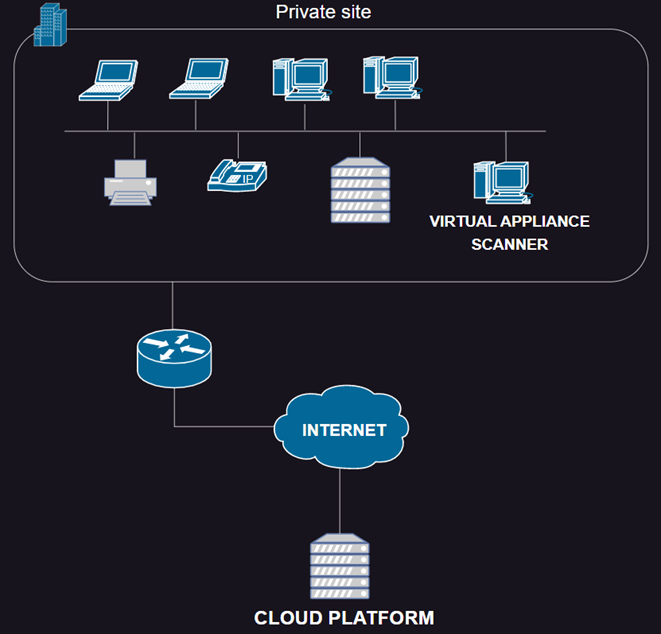
\includegraphics{images/scan_interna.png}
    \caption{Scansione degli asset interni alla rete.}
\end{figure}


Come si evince dall’immagine, la macchina virtuale, oltre ad avere la necessità di accedere alla maggior parte degli asset della rete, ha bisogno di collegarsi a Internet per comunicare con la \textit{cloud platform}. Essa è la piattaforma che gestisce l’intero processo di \textit{vulnerability assessment}, dalla pianificazione e programmazione delle scansioni, alla fase di \textit{remediation} e \textit{patch management}\footnote{Attività periodica di gestione, prioritizzazione, selezione e schedulazione degli aggiornamenti dei software e dei sistemi.}. Una volta installata e configurata la \textit{virtual appliance} è possibile procedere con l’esecuzione della scansione dei \textit{target}.

Il funzionamento di una scansione delle vulnerabilità può essere ridotto al funzionamento di un \textit{port scanner}. Essa infatti esegue una serie di tentativi di connessione con le porte di un sistema, andando quindi a verificare quali servizi sono in ascolto. Poiché un sistema possiede oltre 64.000 porte, risulterebbe molto dispendioso in termini di tempo analizzarle tutte. A questo si aggiunge il fatto che un gran numero di queste porte non viene normalmente utilizzato dai sistemi operativi. Ecco perché il tool di scansione considera principalmente le prime 1024 porte, le cosiddette \textit{well-known ports}. Queste includono, ad esempio, le porte 80 e 443, tipiche dei web server, che offrono servizi in http e https, le porte 22 e 23 che permettono l’accesso remoto al sistema tramite il protocollo sicuro SSH e insicuro Telnet, oppure la porta 21 che identifica il servizio di trasferimento file FTP. Oltre a queste porte è possibile configurare lo scanner in modo che analizzi anche porte specifiche. Se, ad esempio, si vuole verificare l’esposizione di servizi SQL vulnerabili di un database è possibile specificare la porta 3306 per MySQL, oppure la porta 5432 per PostgreSQL.

Una volta identificate le porte in ascolto e stabilita una connessione (nel caso in cui si tratti di porte TCP) lo scanner invia, per ognuna di esse, determinate richieste e comandi. Il comando più semplice che un tool può eseguire è la richiesta del numero di versione del servizio esposto dalla porta in questione. A quel punto il sistema \textit{target} può rispondere alla richiesta normalmente come se il comando fosse eseguito localmente, ad esempio da linea di comando, oppure, se il sistema è configurato a dovere, può rispondere oscurando il riferimento alla versione del servizio. Questo dato può sembrare irrilevante, ma per un ipotetico malintenzionato conoscere la versione dei servizi esposti da un sistema è il primo passo per pianificare l’attacco. Gli \textit{hacker} si muniscono di \textit{toolkit}, ad esempio \textit{metasploit}, che raggruppano insiemi di \textit{exploit} in base alle diverse vulnerabilità note di vari applicativi. Tramite il numero di versione possono quindi identificare, ad esempio con una semplice ricerca in internet, quali vulnerabilità affliggono il servizio in questione. Di conseguenza è possibile risalire relativamente facilmente anche ai rispettivi \textit{exploit} ed eseguire quindi l’attacco.

Si prenda in considerazione lo scenario di un web server Apache pronto a ricevere richieste HTTP o HTTPS. Possiamo collegarci al server con indirizzo IP 172.17.22.233 tramite la porta 80:

\begin{minted}{powershell}
  $ telnet 172.17.22.233 80
\end{minted}

Una volta instaurata la connessione inviamo la seguente richiesta:

\begin{minted}{powershell}
  > HEAD / HTTP/1.0
\end{minted}

E come risposta otteniamo:

\begin{minted}{powershell}
  HTTP/1.1 200 OK
  Date: Fri, 14 Jul 2023 21:23:59 GMT
  Server: Apache/2.4.52 (Ubuntu)
  Last-Modified: Fri, 14 Jul 2023 18:50:47 GMT
  ETag: "29af-60076ed4a731c"
  Accept-Ranges: bytes
  Content-Length: 10671
  Vary: Accept-Encoding
  Connection: close
  Content-Type: text/html
\end{minted}

Come si può notare, in corrispondenza della voce “Server” viene indicata sia la versione del servizio, in questo caso Apache 2.4.52, sia il sistema operativo. Con una semplice modifica al file di configurazione del web server Apache è possibile nascondere questi dati. Ora la risposta alla stessa richiesta è la seguente:

\begin{minted}{powershell}
  HTTP/1.1 200 OK
  Date: Sat, 15 Jul 2023 08:06:19 GMT
  Server: Apache
  Last-Modified: Fri, 14 Jul 2023 18:50:47 GMT
  ETag: "29af-60076ed4a731c"
  Accept-Ranges: bytes
  Content-Length: 10671
  Vary: Accept-Encoding
  Connection: close
  Content-Type: text/html
\end{minted}

Ritornando al funzionamento dello scanner, esso oltre a richiedere generiche informazioni sul servizio, può metterlo alla prova attivamente. Se ad esempio rileva che la porta 139, cioè il servizio NetBIOS\footnote{Network Basic Input/Output System è un protocollo obsoleto per le comunicazioni sulla rete locale solitamente attivo in ambienti Windows.}, è in ascolto, può tentare di effettuare una enumerazione dei nomi dei computer e degli utenti appartenenti al dominio aziendale, o delle cartelle di rete condivise. Ad esempio con il seguente comando:

\begin{minted}{powershell}
  $ nbtscan -v 192.168.1.52
\end{minted}

È possibile visualizzare il nome NetBIOS del target e i suoi servizi disponibili:

\begin{minted}{powershell}
  NetBIOS Name Table for Host 192.168.1.52:
  Name          Service          Type
---------------------------------------------------
  MIRO-PC        <20>           UNIQUE
  MIRO-PC        <00>           UNIQUE
  WORKGROUP      <00>           GROUP
  WORKGROUP      <1e>           GROUP
\end{minted}

Il tag 20 identifica il servizio di condivisione risorse di rete. Lo scanner può quindi andare più a fondo e tentare di verificare se nel \textit{target} è attiva la cosiddetta \textit{null session}, che permette ad un utente remoto di accedere a certe risorse del sistema tramite connessioni anonime, quindi senza username e password, ovvero una sessione nulla:

\begin{minted}{powershell}
  $ smbclient //192.168.1.52/IPC$ -U""

  Anonymous login successful
  Try "help" to get a list of possible commands.
  
  smb: \> ls
  NT_STATUS_ACCESS_DENIED listing \*
\end{minted}

Come si può notare è stato possibile accedere anonimamente alla \textit{share} remota, la quale però, in questo caso, permette giustamente un accesso limitato. L’accesso anonimo, inoltre, permette in alcuni casi, ad esempio se il sistema in oggetto fa parte di un dominio, di enumerare gli username di accesso agli account di tale dominio. Una volta che si conoscono i nomi utente basterà un semplice attacco \textit{brute-force} per trovare uno username con associata una password comune.

Lo strumento di scansione, quindi, a seconda della risposta da parte del \textit{target} a una certa richiesta che mira a verificare la presenza o meno di una falla di sicurezza, classifica il servizio esposto come vulnerabile se tale risposta trova una corrispondenza nel database delle vulnerabilità consultabile nella piattaforma in cloud.

Lo scopo di una scansione esterna (Figura 1.2), invece, è quello di evidenziare le debolezze di un’infrastruttura di rete dal punto di vista di un attaccante posto al di fuori della rete privata aziendale. Si vuole, quindi, valutare la sua sicurezza e la corretta configurazione delle interfacce pubbliche dei dispositivi posti “ai bordi” della rete. Di conseguenza non è possibile giungere a questo obiettivo tramite uno strumento di scansione posto all’interno della rete che si vuole analizzare. La soluzione è utilizzare un \textit{cloud scanner}. Questi strumenti sono programmi in cloud che girano su server esterni di proprietà di aziende specializzate in sicurezza informatica. Nella configurazione di questa tipologia di scansione vengono specificati tutti i possibili \textit{endpoint} della rete in oggetto: gli indirizzi IP delle interfacce pubbliche di firewall e router, eventuali collegamenti a VPN e riferimenti di possibili server esposti in rete.

%Di seguito uno schema di tale concetto.

\begin{figure}[h]
\centering
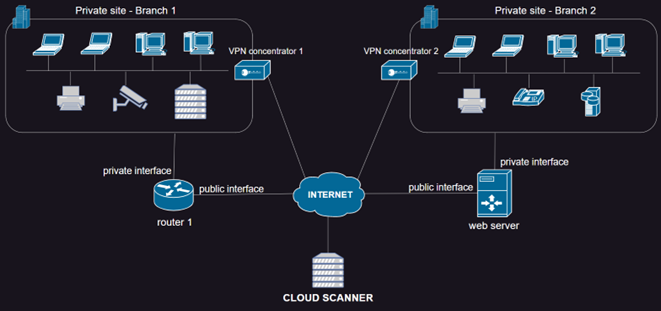
\includegraphics[scale=1.2]{images/scan_esterna.png}
    \caption{Scansione degli asset ai confini della rete.}
\end{figure}


Tramite questa architettura la piattaforma esterna in cloud è in grado di interrogare gli apparati di rete sulle loro interfacce pubbliche. Solitamente vengono rilevate configurazioni deboli come l’utilizzo di protocolli di sicurezza obsoleti oppure generiche vulnerabilità di server esposti.

Finora abbiamo preso in considerazione le scansioni \textit{agentless}, ovvero quelle scansioni che vengono eseguite attivamente da uno strumento di analisi, sia esso una \textit{virtual appliance} o un \textit{cloud scanner}. Esistono però anche le scansioni basate sui cosiddetti agenti. Una configurazione \textit{agent-based} consiste nell’avere per ogni \textit{host target} (oppure per i più critici) un software (o endpoint) chiamato agente installato localmente nella macchina. Questo programma raccoglie in tempo reale i parametri del sistema, l’utilizzo delle risorse, i software installati, le connessioni di rete e gli eventi più sospetti. Oltre a queste informazioni, l’agente, come un qualsiasi software antivirus, effettua periodiche scansioni del sistema sul quale è installato. Un grande vantaggio di questa soluzione consiste nell’avere per ogni asset report più accurati e meno falsi negativi, inoltre le analisi possono essere effettuate in autonomia dalle singole macchine senza compromettere la disponibilità della rete. Ulteriore vantaggio da questa soluzione si ha quando l’azienda permette di ospitare, magari occasionalmente, dispositivi non gestiti, ad esempio i cosiddetti BYOD (\textit{Bring Your Own Device}). Questi dispositivi sono una reale minaccia per la rete aziendale in quanto sono devices non monitorati ad uso personale e molto spesso contengono software non aggiornati e vulnerabili. Risulta quindi evidente che una valutazione periodica \textit{agentless} dell’infrastruttura non sia ottimale in questo caso. È plausibile infatti che durante tali scansioni non sempre questi dispositivi siano presenti fisicamente nella rete aziendale e che quindi non sia possibile valutarne e correggerne le vulnerabilità. Per questo motivo, in scenari come quello appena illustrato, conviene tenere in considerazione le scansioni basate sugli agenti. Idealmente una scansione per le vulnerabilità dovrebbe consistere in un approccio ibrido: imbastire una scansione \textit{agentless} in modo da valutare lo stato generale della rete, permettendo anche di rilevare e analizzare asset che non erano stati presi in considerazione; predisporre per gli asset più sensibili ed esposti a rischi delle scansioni \textit{agent-based}.

I dati raccolti dalle scansioni vengono poi inviati alla piattaforma in cloud e processati in report.

\section{Analisi dei risultati}
Senza un’accurata ispezione dei risultati, prima di presentarli al committente, il \textit{vulnerability assessment} avrebbe un valore molto limitato. Al termine delle scansioni lo strumento di analisi genera automaticamente un report per ogni attività, che prende il nome di \textit{technical report}. Questi documenti raccolgono, per ogni \textit{subnet} analizzata, tutte le informazioni e i dati utili rilevati sui singoli dispositivi. Tra questi vi sono, oltre al numero di vulnerabilità suddiviso per criticità e tipologia e le rispettive descrizioni, riferimenti ai sistemi operativi rilevati e ai servizi attivi in ascolto. Tali report, in quanto generati in automatico, necessitano di essere revisionati accuratamente per verificare eventuali inesattezze o imprecisioni. Come in qualsiasi attività di testing, infatti, è molto probabile che possano essere presenti falsi positivi. Prendiamo, ad esempio, in considerazione lo scenario in cui un web server venga interrogato dal \textit{vulnerability scanner}. Quest’ultimo, a seconda del payload che invia, si aspetta una determinata risposta da parte del server se questo è vulnerabile. Tuttavia, se la risposta è ambigua o non rientra tra gli scenari che il tool di scansione si aspetterebbe, lo scanner potrebbe classificare in modo inesatto il server. Esso, ad una determinata richiesta, potrebbe smettere di rispondere quando al contrario lo scanner si aspetterebbe una risposta, per esempio un messaggio di errore nel caso in cui non fosse vulnerabile. Come interpretare questa assenza di risposta? La \textit{query} dello scanner potrebbe aver causato un’interruzione del servizio e quindi il server sarebbe vulnerabile ad attacchi di tipo \textit{Denial of Service}. Tuttavia, il server potrebbe aver deciso di interrompere la connessione seguendo un meccanismo di difesa implementato ad esempio dall’amministratore di sistema. In questi casi lo strumento di scansione interpreterà l’evento ipotizzando lo scenario peggiore e classificherà il \textit{target} come vulnerabile. È preferibile, infatti, avere falsi positivi rispetto a rischiare di ignorare una possibile vulnerabilità. Altro rumore di fondo ricorrente nei report generati è dovuto alla valutazione della validità dei certificati SSL installati sui dispositivi. Ovviamente è corretto che lo scanner identifichi e controlli la validità di un certificato, quindi che esso risulti emesso da un’autorità attendibile o che non sia scaduto. A nessuna azienda farebbe piacere ricevere segnalazioni dai propri clienti riguardo a problemi di accesso e avvisi di sicurezza del proprio sito web. Diversa invece è la questione quando si tratta di certificati \textit{self-signed} installati in quei dispositivi di gestione come router, firewall, switch ecc. ai quali si può accedere solo dalla rete locale interna. Questi dispositivi possiedono un certificato auto generato ma, dato che solitamente l’accesso a tali dispositivi viene effettuato direttamente tramite indirizzo IP, l’errore che il browser propone può essere ignorato, in quanto siamo consapevoli che stiamo contattando il dispositivo con quello specifico indirizzo. Inoltre non vi è nemmeno il rischio di intercettazione di informazioni in chiaro, in quanto se il dispositivo possiede un certificato correttamente installato ed è configurato per rispondere in \textit{https}, la connessione viene crittografata pur trattandosi di un certificato non riconosciuto. Data la quantità di dispositivi di gestione presenti in una rete aziendale, si può immaginare quanto “rumore” essi possano causare in un \textit{technical report}. È per questo che è importante usare i risultati delle prime scansioni per affinare e calibrare lo strumento aggiungendo nella sua configurazione eventuali eccezioni. Nel seguito questo aspetto verrà illustrato più in dettaglio.

Il lavoro dell’analista è quindi quello di interpretare, nel modo più oggettivo possibile, i risultati ottenuti riportandoli in un \textit{executive report}, il documento che verrà presentato al cliente. L’analista, oltre a dover discernere ciò che è irrilevante e fuorviante da ciò che necessita realmente di attenzione, deve contestualizzare i risultati restando il più possibile attinente alle informazioni oggettive ottenute dal \textit{technical report}. Il documento, infatti, verrà consultato anche dall’eventuale reparto IT dell’azienda cliente. Dato che solo loro possiedono il preciso quadro generale della propria infrastruttura, sbilanciarsi con certe supposizioni riguardo ad esempio una composizione non ottimale della rete, oppure l’identificazione di una precisa tipologia di dispositivo, rischia di invalidare il lavoro svolto portando a delle conclusioni false e a una cattiva reputazione agli occhi dell’azienda cliente. Non bisogna dimenticare che, a meno di specifiche configurazioni, lo scanner di rete non ha alcuna conoscenza riguardo l’infrastruttura in questione e ogni informazione che rileva è basata esclusivamente dalle corrispondenze che individua tra le risposte dei \textit{target} e quelle contenute in un database limitato.

I risultati delle analisi dovranno essere esposti anche al personale amministrativo. L’analista deve riportare i risultati nell’\textit{executive report} in linguaggio naturale limitando i termini tecnici. Il documento dovrà quindi essere comprensibile da persone non esperte e illustrerà, anche per mezzo di grafici, per ogni \textit{subnet} analizzata, la relativa situazione in termini di numero, criticità e distribuzione delle vulnerabilità. Insieme a una breve descrizione delle criticità più rilevanti, vengono date delle possibili soluzioni per porne rimedio.

\section{Remediation}

Un’esecuzione periodica del \textit{vulnerability assessment} permette di identificare prima di un potenziale malintenzionato le criticità maggiori all’interno e all’esterno della rete aziendale. La fase di risoluzione di tali criticità è un altrettanto regolare processo di indagine e documentazione degli asset vulnerabili più esposti. Il documento riepilogativo, stilato nella fase di analisi dei risultati, permette ai tecnici e ai manager di avere una visione di insieme riguardo gli asset e le sottoreti più a rischio e considerare quindi le migliori soluzioni, anche a lungo termine. Al termine di ogni descrizione delle risultanze trovate nei \textit{target} viene presentata una loro possibile risoluzione. Nell’\textit{executive report} questa consiste in una spiegazione sintetica, mentre il \textit{technical report} dato in mano al reparto IT aziendale presenta le problematiche e le relative risoluzioni in modo più specifico e pratico, con riferimenti alla documentazione ufficiale dei servizi in uso.

Le vulnerabilità sono classificate in base alla loro severità, seguendo una serie di metriche che verranno presentate nel seguito. Vulnerabilità con \textit{severity} bassa e media non presentano un rischio diretto per la sicurezza dell’infrastruttura aziendale, ma se sfruttate potrebbero rivelare informazioni utili a un potenziale attaccante per la pianificazione ed esecuzione di un attacco. Le vulnerabilità di livello alto e critico invece necessitano di interventi tempestivi in quanto il loro \textit{exploit} permette gravi compromissioni alla confidenzialità, integrità o disponibilità della rete.

Idealmente la fase di \textit{remediation} dovrebbe porre rimedio a tutte quelle vulnerabilità che presentano un livello di rischio considerevole. Nel seguito verranno presentate le tipologie di vulnerabilità che richiedono maggiore attenzione. Nella pratica, eliminare e isolare più falle possibili richiede un’accurata analisi dei sistemi attivi, dei rispettivi servizi esposti sia verso la rete pubblica che nella intranet aziendale e delle politiche di visibilità e connessione tra le varie \textit{subnet} aziendali. Porre rimedio alle debolezze trovate durante l’analisi vuol dire anche trovare dei compromessi fra la praticità e la comodità di utilizzo dei sistemi con i quali ci si interfaccia e la loro conformità dal punto di vista della sicurezza. Si pensi ad esempio all’implementazione di meccanismi di autenticazione a doppio fattore\footnote{Meccanismo che in fase di autenticazione a un servizio richiede, oltre a username e password, l'inserimento di un codice temporaneo generato da un proprio dispositivo mobile in modo da dimostrare il suo possesso.} o all’introduzione di politiche più stringenti in merito ai comportamenti ai quali gli utenti finali devono attenersi. Altri compromessi possono riguardare cali di \textit{performance} della rete a seguito dell’installazione di dispositivi e/o software di analisi e scansione dei pacchetti di rete delle connessioni in entrata e in uscita.

Per tenere traccia dei progressi, in termini di risoluzione delle problematiche, vengono stilati i \textit{vulnerability assessment} 
comparativi. Questi documenti prendono in considerazione due o più periodi nei quali si è svolta una valutazione della sicurezza e li compara con i risultati dell’ultima esecuzione di un \textit{vulnerability assessment}. Questo permette di avere uno storico dettagliato con quantità e tipologia di vulnerabilità e di dispositivi affetti potendo metterlo in relazione con la rilevazione più recente e valutando quindi l’operato e gli sforzi dell’azienda nella messa in sicurezza degli \textit{asset} più esposti e vulnerabili.

Infine tutti i documenti redatti, ad eccezione del \textit{technical report}, vengono discussi insieme al committente e al responsabile del reparto IT.

\chapter{Caso di studio: analisi delle vulnerabilità di una rete aziendale}
In questo capitolo si espone un caso di studio reale di esecuzione di un \textit{vulnerability assessment} per un'azienda metalmeccanica che produce componenti per il settore dell'Automotive.

La scansione è stata eseguita nel febbraio 2023 e fa parte della commessa richiesta dall'azienda per la valutazione della sicurezza della rete, che prevede, oltre al \textit{vunerability assessment}, attività di \textit{penetration test} e campagne di \textit{phishing}\footnote{k}. 

\section{Strumentazione}
Esistono un gran numero di \textit{vulnerability scanning tools} che differiscono, oltre che per il prezzo , in base alle tecnologie che supportano (oltre a Windows, Linux e macOS potrebbero esserci sistemi insoliti per i quali lo scanner non è stato programmato), se sono dedicati anche alle \textit{web applications scans}  e in base ad eventuali configurazioni come il grado di automazione e la possibilità di schedulare le scansioni. La maggior parte dei tool di scansione però consiste in software accessibili da piattaforme in cloud attraverso il browser.

Nel nostro caso si è impiegato lo strumento Qualys VMDR (Vulnerability Management, Detection, and Response). Nell'appendice \ref{appendix:a} viene illustrato come si presenta il software.

Tramite la sua interfaccia è possibile avere una panoramica delle scansioni già eseguite, in esecuzione o programmate e delle vulnerabilità trovate più di frequente, è possibile consultare i \textit{technical} ed \textit{executive} report e creare dei piani di \textit{remediation}. Fondamentale è anche la possibilità di consultare il database costantemente aggiornato delle ultime vulnerabilità pubblicate.

È possibile inoltre organizzare gli asset in gruppi che andranno a definire i \textit{target} della scansione. Figura \ref{fig:qualys_targets}.

\section{\textit{Target definition}}
Lo \textit{scope} della scansione viene definito dal cliente e, insieme al reparto IT, vengono comunicate tutte le \textit{subnet} da includere, o le più prioritarie. La lista seguente definisce le sottoreti che saranno oggetto della scansione:

%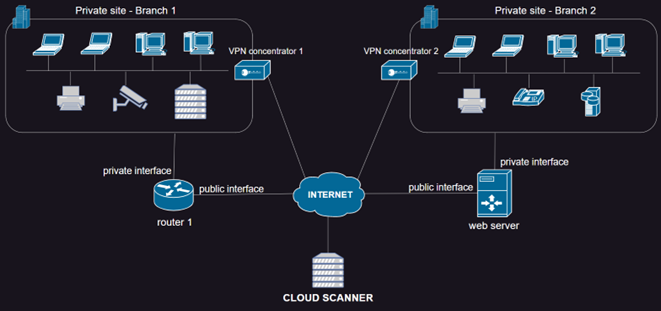
\includegraphics[scale=1.2]{images/scan_esterna.png}

%% Fine dei capitoli normali, inizio dei capitoli-appendice (opzionali)
\appendix

%\part{Appendici}

\chapter{Interfacce di Qualys}
\label{appendix:a}

\begin{figure}
\centering
    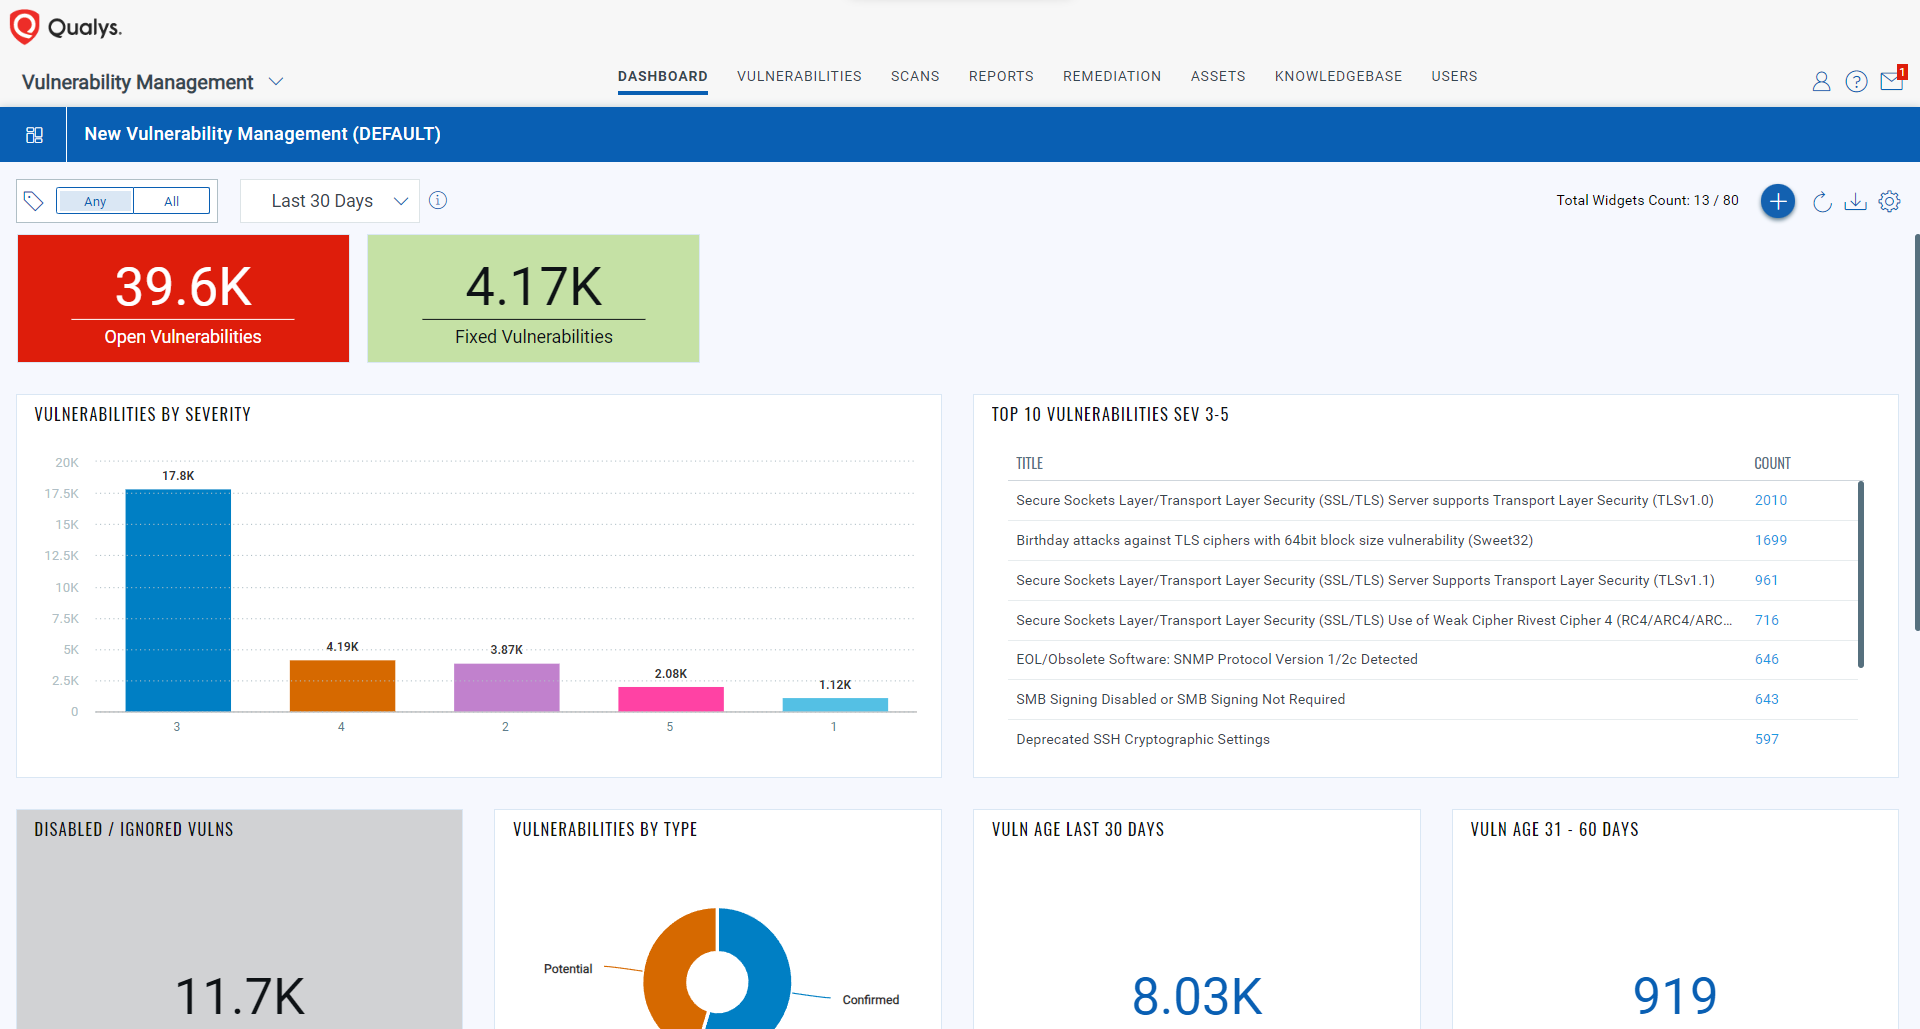
\includegraphics[scale=0.329]{images/qualys_dashboard.png}
    \caption{\textit{Dashboard}. Visualizza una panoramica, personalizzabile attraverso \textit{widget}, dei risultati e dell'andamento delle scansioni eseguite.}
\end{figure}

\begin{figure}
\centering
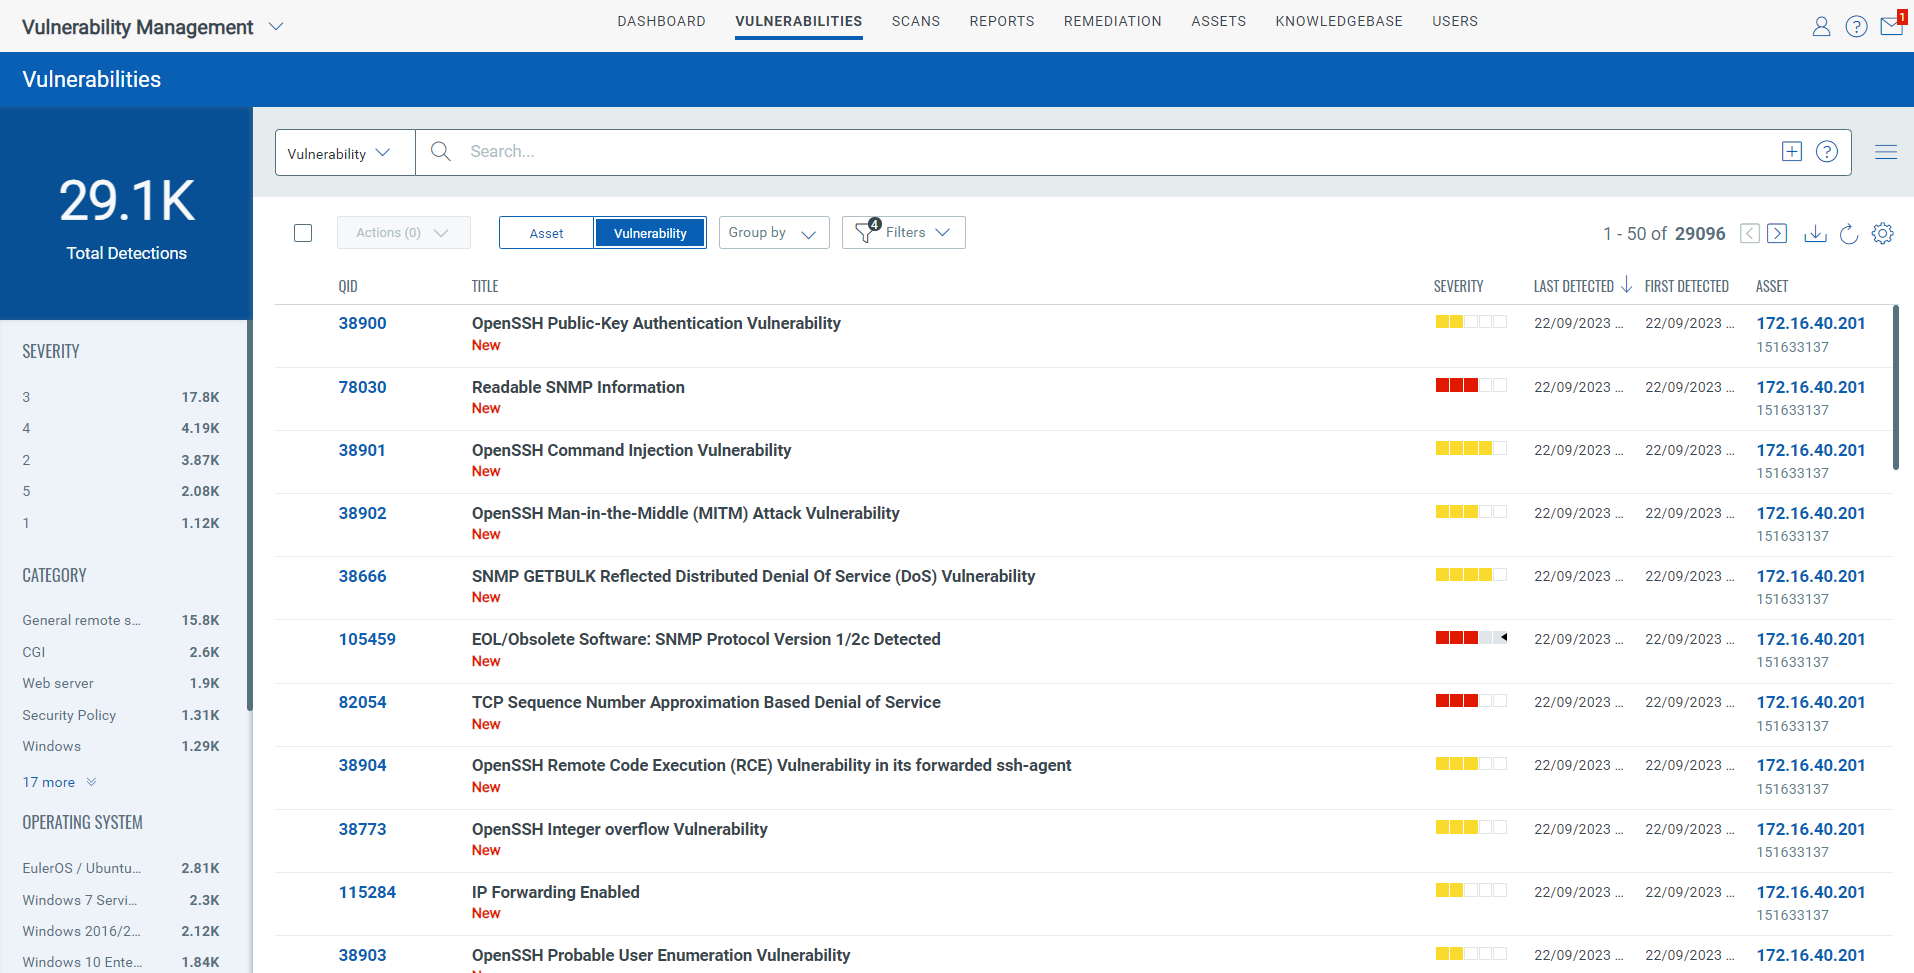
\includegraphics[scale=0.329]{images/qualys_vuln.png}
    \caption{\textit{Vulnerabilities}. Visualizza una lista delle vulnerabilità trovate nelle ultime scansioni effettuate.}
\end{figure}

\begin{figure}
\centering
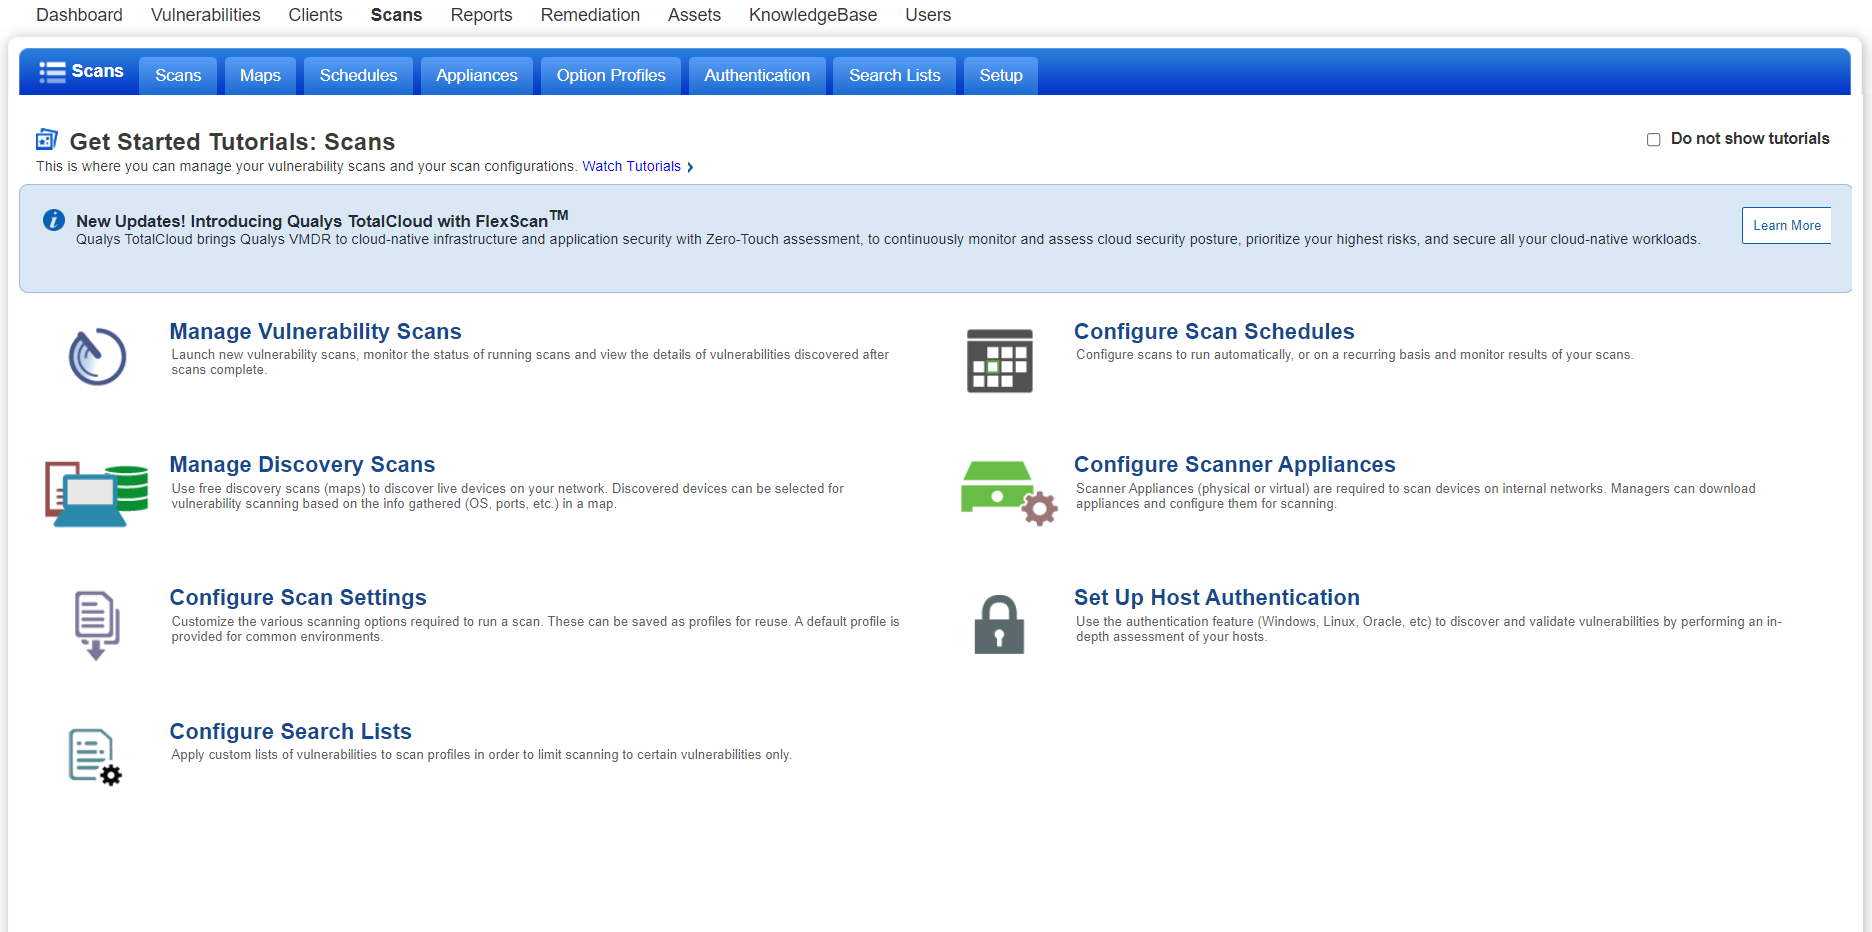
\includegraphics[scale=0.329]{images/qualys_scans.png}
    \caption{\textit{Scans}. Da qui è possibile configurare, schedulare e monitorare l'esecuzione delle scansioni vere e proprie.}
\end{figure}

\begin{figure}
\centering
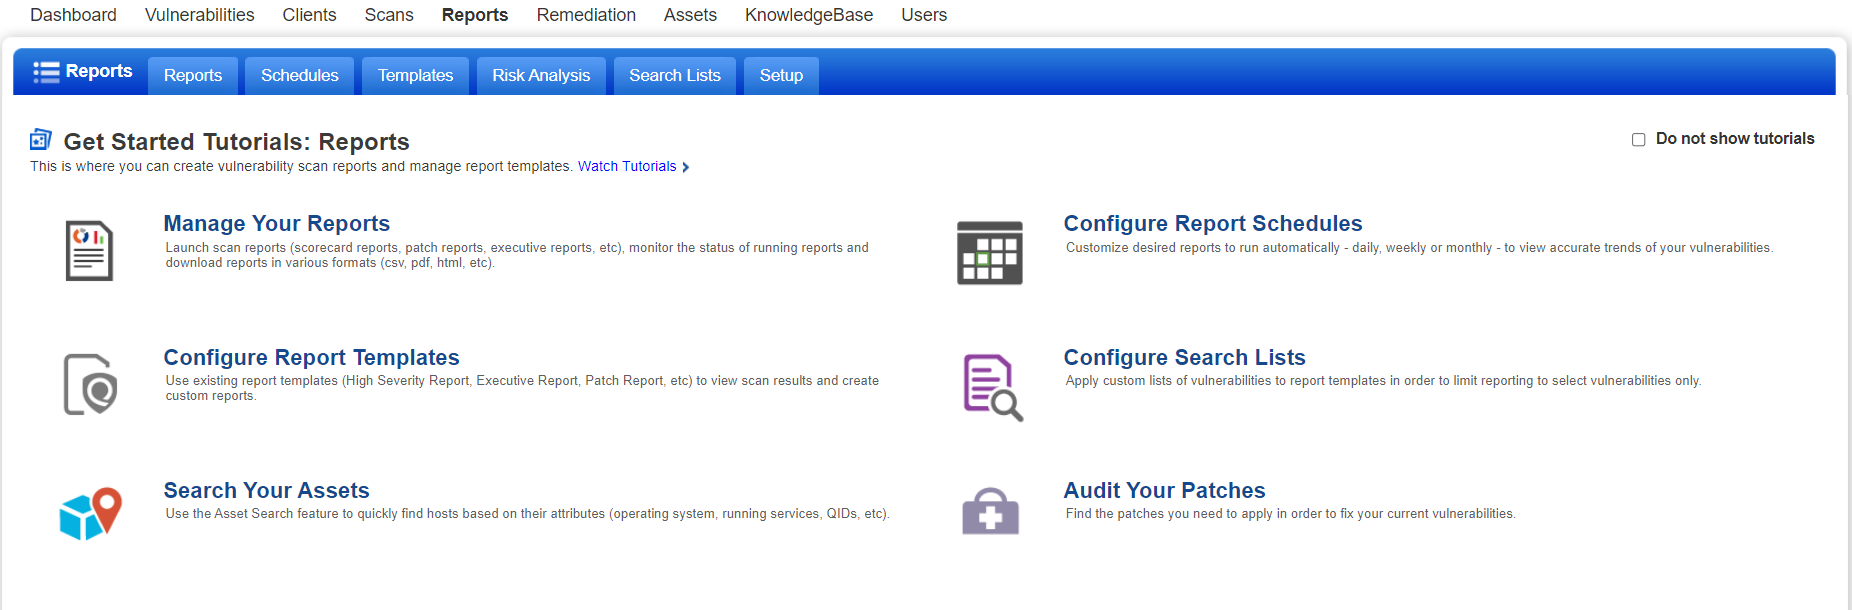
\includegraphics[scale=0.329]{images/qualys_reports.png}
    \caption{\textit{Reports}. Questa sezione permette di visualizzare i report generati dalle scansioni oppure generarne manualmente. È possibile anche personalizzare i \textit{template} con i quali vengono generati i report.}
\end{figure}

\begin{figure}
\centering
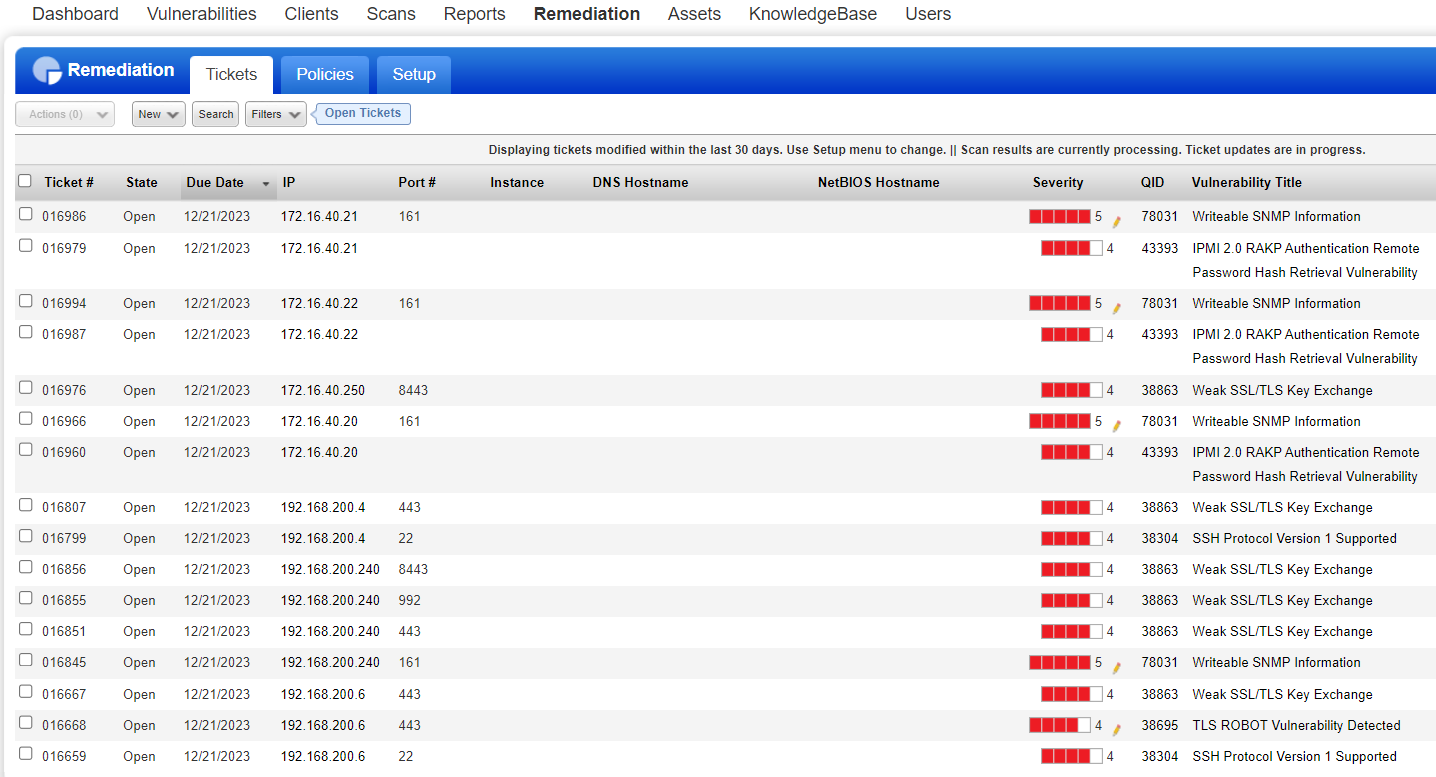
\includegraphics[scale=0.425]{images/qualys_remediation.png}
    \caption{\textit{Remediation}. Visualizza la lista, con le relative scadenze di risoluzione, delle vulnerabilità trovate e non ancora risolte.}
\end{figure}

\begin{figure}
\centering
\includegraphics[scale=0.329]{images/qualys_assets.png}
    \caption{\textit{Assets}. Permette di creare e gestire gli asset e i relativi gruppi che saranno oggetto delle scansioni.}
\end{figure}

\begin{figure}
    \centering
    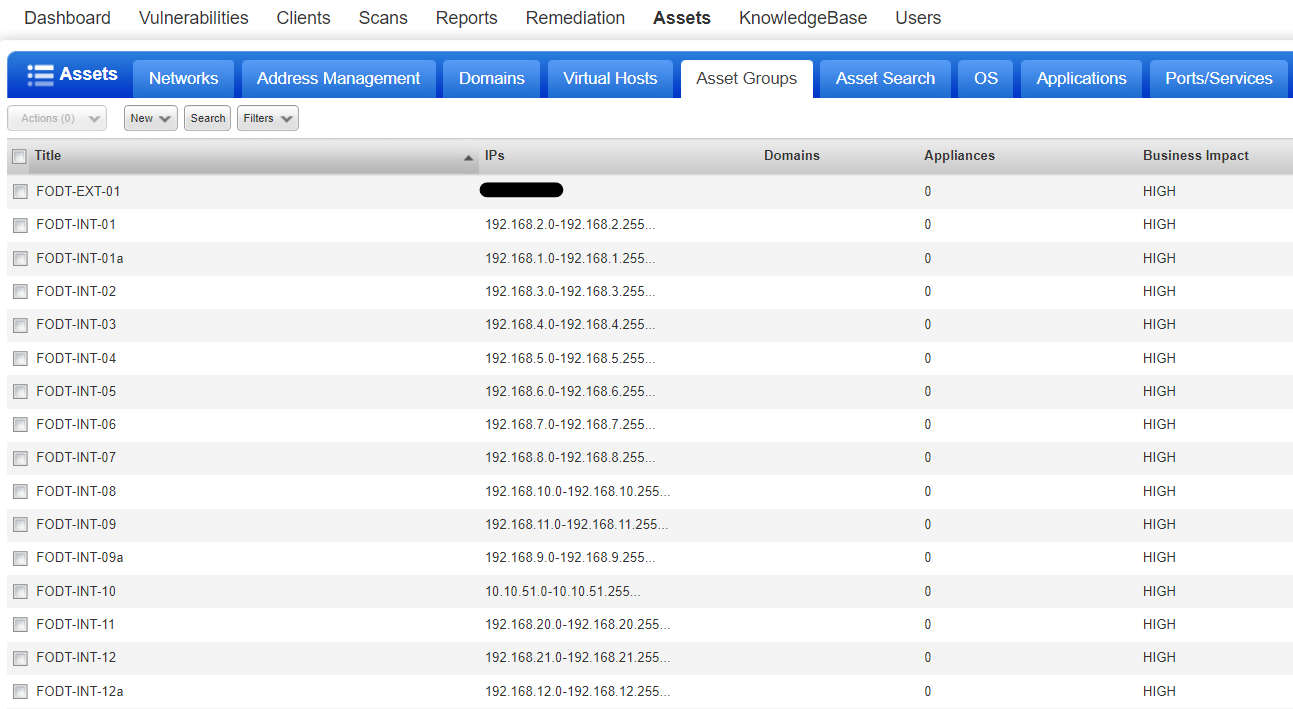
\includegraphics[width=1\linewidth]{images/qualys_targets.png}
    \caption{Lista degli \textit{asset groups}. Ogni gruppo è costituito da indirizzi IP singoli, intervalli o \textit{subnet} intere, o da specifici domini.}
    \label{fig:qualys_targets}
\end{figure}

\begin{figure}
\centering
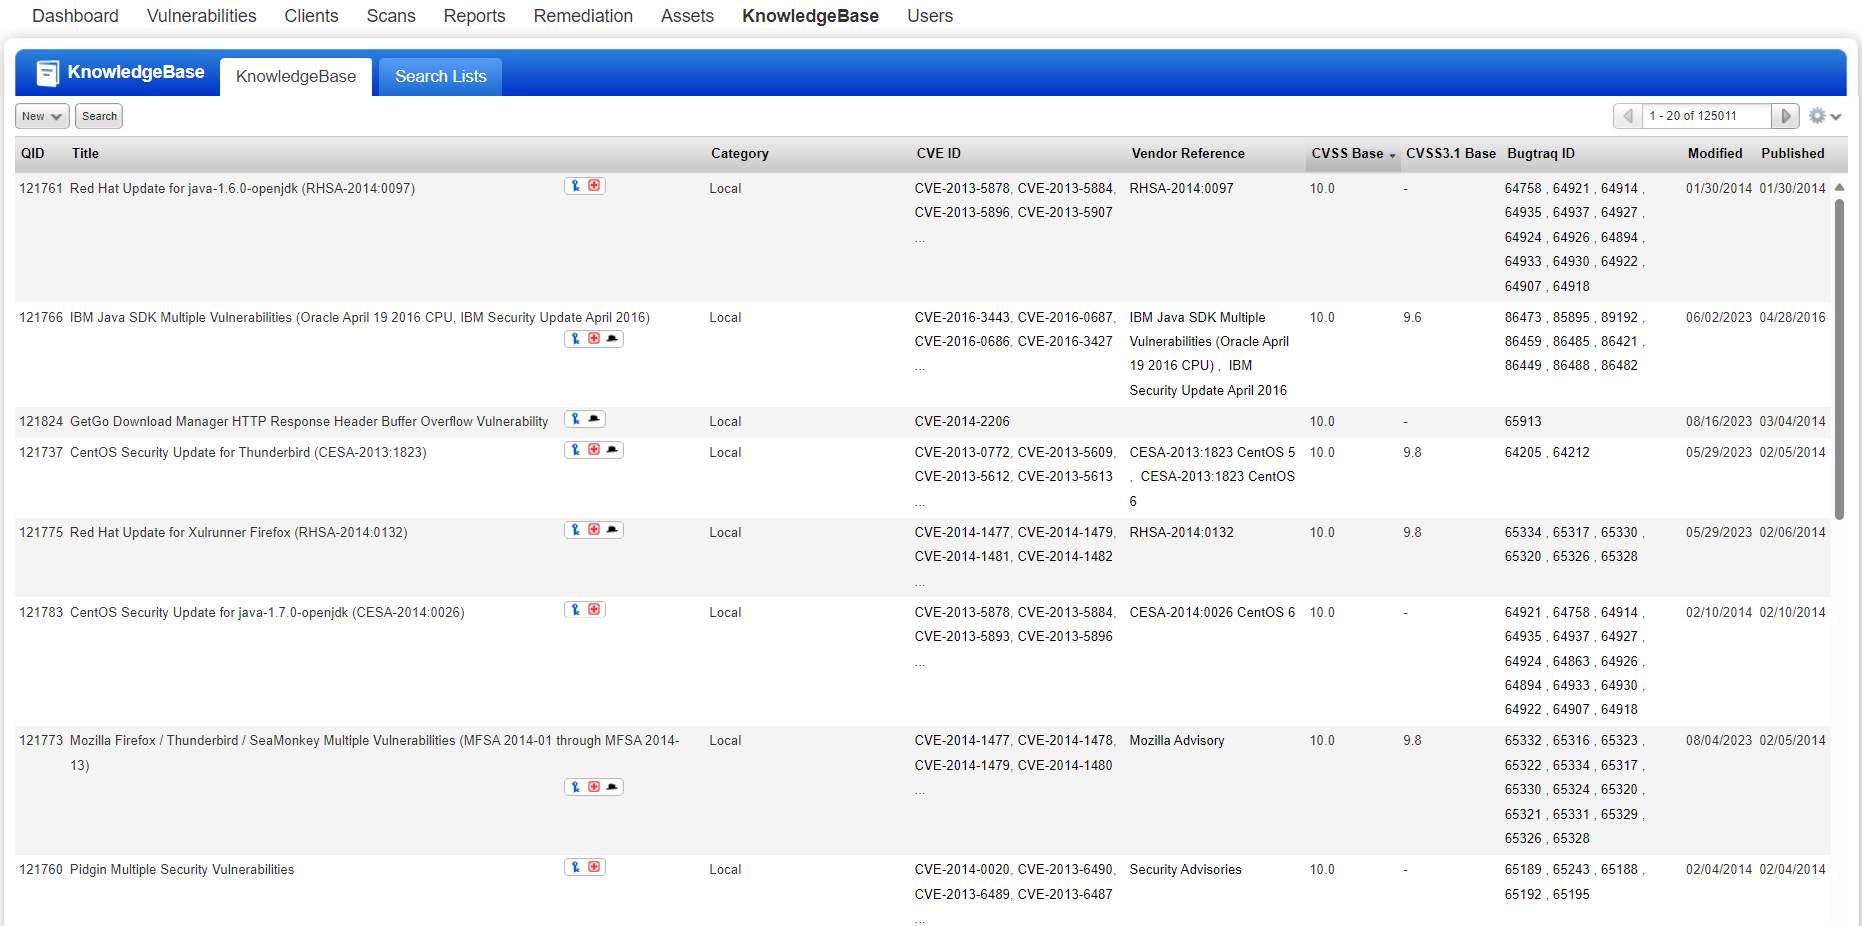
\includegraphics[scale=0.35]{images/qualys_kb.png}
    \caption{\textit{Knowledgebase}. Questo è il database delle vulnerabilità proprietario di \textit{Qualys} costantemente aggiornato. È possibile, per ogni voce, aggiungere commenti che verranno visualizzati nei report, modificare il livello di criticità delle vulnerabilità o disabilitarle in modo che le scansioni le ignorino.}
\end{figure}

%% Parte conclusiva del documento; tipicamente per riassunto, bibliografia e/o indice analitico.
\backmatter

%% Riassunto (opzionale)
%\summary
%Maecenas tempor elit sed arcu commodo, dapibus sagittis leo egestas. Praesent at ultrices urna. Integer et nibh in augue mollis facilisis sit amet eget magna. Fusce at porttitor sapien. Phasellus imperdiet, felis et molestie vulputate, mauris sapien tincidunt justo, in lacinia velit nisi nec ipsum. Duis elementum pharetra lorem, ut pellentesque nulla congue et. Sed eu venenatis tellus, pharetra cursus felis. Sed et luctus nunc. Aenean commodo, neque a aliquam bibendum, mauris augue fringilla justo, et scelerisque odio mi sit amet diam. Nulla at placerat nibh, nec rutrum urna. Donec ut egestas magna. Aliquam erat volutpat. Phasellus vestibulum justo sed purus mattis, vitae lacinia magna viverra. Nulla rutrum diam dui, vel semper mi mattis ac. Vestibulum ante ipsum primis in faucibus orci luctus et ultrices posuere cubilia Curae; Donec id vestibulum lectus, eget tristique est.

%% Bibliografia (praticamente obbligatoria)
\bibliographystyle{plain_\languagename}%% Carica l'omonimo file .bst, dove \languagename è la lingua attiva.
%% Nel caso in cui si usi un file .bib (consigliato)
\bibliography{thud}
%% Nel caso di bibliografia manuale, usare l'environment thebibliography.

%% Per l'indice analitico, usare il pacchetto makeidx (o analogo).

\end{document}
